\documentclass[dvipdfmx]{jsarticle}
\setcounter{section}{2}
\setcounter{subsection}{3}
\usepackage{amsmath,amsfonts,amssymb,array,comment,mathtools,url,docmute}
\usepackage{longtable,booktabs,dcolumn,tabularx,mathtools,multirow,colortbl,xcolor}
\usepackage[dvipdfmx]{graphics}
\usepackage{bmpsize}
\usepackage{amsthm}
\usepackage{enumitem}
\setlistdepth{20}
\renewlist{itemize}{itemize}{20}
\setlist[itemize]{label=•}
\renewlist{enumerate}{enumerate}{20}
\setlist[enumerate]{label=\arabic*.}
\setcounter{MaxMatrixCols}{20}
\setcounter{tocdepth}{3}
\newcommand{\rotin}{\text{\rotatebox[origin=c]{90}{$\in $}}}
\renewcommand{\thesection}{第\arabic{section}部}
\renewcommand{\thesubsection}{\arabic{section}.\arabic{subsection}}
\renewcommand{\thesubsubsection}{\arabic{section}.\arabic{subsection}.\arabic{subsubsection}}
\everymath{\displaystyle}
\allowdisplaybreaks[4]
\usepackage{vtable}
\theoremstyle{definition}
\newtheorem{thm}{定理}[subsection]
\newtheorem*{thm*}{定理}
\newtheorem{dfn}{定義}[subsection]
\newtheorem*{dfn*}{定義}
\newtheorem{axs}[dfn]{公理}
\newtheorem*{axs*}{公理}
\renewcommand{\headfont}{\bfseries}
\makeatletter
  \renewcommand{\section}{%
    \@startsection{section}{1}{\z@}%
    {\Cvs}{\Cvs}%
    {\normalfont\huge\headfont\raggedright}}
\makeatother
\makeatletter
  \renewcommand{\subsection}{%
    \@startsection{subsection}{2}{\z@}%
    {0.5\Cvs}{0.5\Cvs}%
    {\normalfont\LARGE\headfont\raggedright}}
\makeatother
\makeatletter
  \renewcommand{\subsubsection}{%
    \@startsection{subsubsection}{3}{\z@}%
    {0.4\Cvs}{0.4\Cvs}%
    {\normalfont\Large\headfont\raggedright}}
\makeatother
\makeatletter
\renewenvironment{proof}[1][\proofname]{\par
  \pushQED{\qed}%
  \normalfont \topsep6\p@\@plus6\p@\relax
  \trivlist
  \item\relax
  {
  #1\@addpunct{.}}\hspace\labelsep\ignorespaces
}{%
  \popQED\endtrivlist\@endpefalse
}
\makeatother
\renewcommand{\proofname}{\textbf{証明}}
\usepackage{tikz,graphics}
\usepackage[dvipdfmx]{hyperref}
\usepackage{pxjahyper}
\hypersetup{
 setpagesize=false,
 bookmarks=true,
 bookmarksdepth=tocdepth,
 bookmarksnumbered=true,
 colorlinks=false,
 pdftitle={},
 pdfsubject={},
 pdfauthor={},
 pdfkeywords={}}
\begin{document}
%\hypertarget{ux5546ux96c6ux5408}{%
\subsection{商集合}%\label{ux5546ux96c6ux5408}}
\subsubsection{関係}%\label{ux95a2ux4fc2}}
\begin{dfn}
集合たち$A$、$B$が与えられたとする。このとき、$R = (A \times B,G):A \multimap B$なる対応$R$を考えると、その値域$V\left( R \middle| \left\{ a \right\} \right)$が空集合でないとき、対応の定義より次式が成り立つような元$b$がその集合$A$に存在する。
\begin{align*}
b \in V\left( R \middle| \left\{ a \right\} \right) \subseteq B
\end{align*}
このことを$aRb$と書きその対応$R$をその集合$A$からその集合$B$への関係といい、これのgraph$G$をその関係$R$のgraphといい$G(R)$とも書く。特に、$A = B$のとき、その関係$R$はその集合$A$における関係という。例えば、等号$=$、必要十分条件$\Leftrightarrow$などが挙げられる。
\end{dfn}
\begin{axs}
次のことを満たすような関係$R$をその集合$A$における同値関係という。
\begin{itemize}
\item
  その関係$R$は反射的である、即ち、$\forall a \in A$に対し、$aRa$が成り立つ。
\item
  その関係$R$は対称的である、即ち、$\forall a,b \in A$に対し、$aRb \Leftrightarrow bRa$が成り立つ。
\item
  その関係$R$は推移的である、即ち、$\forall a,b,c \in A$に対し、$aRb \land bRc \Rightarrow aRc$が成り立つ。
\end{itemize}
集合$A$における同値関係$R$が与えられたとき、$aRb$なるその集合$A$の2つの元々$a$、$b$はその同値関係$R$に関して同値であるという。
\end{axs}
\begin{axs}
次のことを満たすような関係$R$をその集合$A$における半順序関係、または単に、順序関係という。
\begin{itemize}
\item
  その関係$R$は反射的である、即ち、$\forall a \in A$に対し、$aRa$が成り立つ。
\item
  その関係$R$は反対称的である、即ち、$\forall a,b \in A$に対し、$aRb \land bRa \Rightarrow a = b$が成り立つ。
\item
  その関係$R$は推移的である、即ち、$\forall a,b,c \in A$に対し、$aRb \land bRc \Rightarrow aRc$が成り立つ。
\end{itemize}
\end{axs}
\begin{axs}
次のことを満たすような関係$R$をその集合$A$における全順序関係という。
\begin{itemize}
\item
  その関係$R$は反射的である、即ち、$\forall a \in A$に対し、$aRa$が成り立つ。
\item
  その関係$R$は反対称的である、即ち、$\forall a,b \in A$に対し、$aRb \land bRa \Rightarrow a = b$が成り立つ。
\item
  その関係$R$は推移的である、即ち、$\forall a,b,c \in A$に対し、$aRb \land bRc \Rightarrow aRc$が成り立つ。
\item
  その関係$R$は全順序的である、即ち、$\forall a,b \in A$に対し、$aRb \vee bRa$が成り立つ。
\end{itemize}
\end{axs}
\begin{thm}\label{1.2.5.6}
集合$A$から集合$B$への関係たち$R$、$S$が与えられたとき、$\forall a \in A\forall b \in B$に対し、$aRb \Leftrightarrow aSb$が成り立つならそのときに限り、$R = S$が成り立つ。
\end{thm}
\begin{proof}
集合$A$から集合$B$への関係たち$R$、$S$が与えられたとき、$\forall a \in A\forall b \in B$に対し、$aRb \Leftrightarrow aSb$が成り立つなら、次式が成り立つ。
\begin{align*}
b \in V\left( R|\left\{ a \right\} \right) \Leftrightarrow b \in V\left( S|\left\{ a \right\} \right)
\end{align*}
これはそれらの同値関係たち$R$、$S$のgraphsをそれぞれ$G(R)$、$G(S)$とおくと、次式のように書き換えられることができる。
\begin{align*}
b \in A \land \exists a' \in \left\{ a \right\}\left[ \left( a',b \right) \in G(R) \right] \Leftrightarrow b \in A \land \exists a' \in \left\{ a \right\}\left[ \left( a',b \right) \in G(S) \right]
\end{align*}
したがって、次のようになる。
\begin{align*}
&\quad \left( b \in A \land \exists a' \in \left\{ a \right\}\left[ \left( a',b \right) \in G(R) \right] \Leftrightarrow b \in A \land \exists a' \in \left\{ a \right\}\left[ \left( a',b \right) \in G(S) \right] \right)\\
&\Leftrightarrow \left( a,b \in A \land (a,b) \in G(R) \Leftrightarrow a,b \in A \land (a,b) \in G(S) \right)\\
&\Leftrightarrow \left( a,b \in A \land (a,b) \in G(R) \land (a,b) \in G(S) \right) \\
&\quad \vee \left( \neg a,b \in A \vee (a,b) \notin G(R) \vee (a,b) \notin G(S) \right)\\
&\Leftrightarrow \left( (a,b \in A \vee \neg a,b \in A) \land \left( \left( (a,b) \in G(R) \land (a,b) \in G(S) \right) \vee \neg a,b \in A \right) \right) \\
&\quad \vee \left( (a,b) \notin G(R) \vee (a,b) \notin G(S) \right)\\
&\Leftrightarrow \left( (a,b) \in G(R) \land (a,b) \in G(S) \right) \vee \left( (a,b) \notin G(R) \vee (a,b) \notin G(S) \right)\\
&\Leftrightarrow \left( (a,b) \in G(R) \Leftrightarrow (a,b) \in G(S) \right)
\end{align*}
これにより、$G(R) = G(S)$が成り立つので、$\left( A \times B,G(R) \right) = \left( A \times B,G(S) \right)$が成り立ち$R = S$が得られた。\par
逆に、$R = S$が成り立つなら、明らかに$\forall a \in A\forall b \in B$に対し、$aRb \Leftrightarrow aSb$が成り立つ。
\end{proof}
\begin{thm}\label{1.2.5.7}
ここで、写像$f:A \rightarrow B$が与えられたとする。このとき、その集合$A$の元々$a$、$b$に対し、次式のように論理式$aR(f)b$が定義されると、
\begin{align*}
aR(f)b \Leftrightarrow a,b \in A \land f(a) = f(b)
\end{align*}
その集合$A$における関係$R(f)$が得られこれは同値関係となる。
\end{thm}
\begin{dfn}
この関係$R(f)$をその写像$f$に付随する同値関係、その写像$f$の同値核などという。
\end{dfn}
\begin{proof}
写像$f:A \rightarrow B$が与えられたとする。このとき、その集合$A$の元々$a$、$b$に対し、次式のように論理式$aR(f)b$が定義されるとする。
\begin{align*}
aR(f)b \Leftrightarrow a,b \in A \land f(a) = f(b)
\end{align*}
このとき、次式のようなその集合$A \times A$の部分集合$G$が定義されると、
\begin{align*}
G = \left\{ (a,b) \in A^{2} \middle| f(a) = f(b) \right\}
\end{align*}
$R = (A,A,G):A \multimap A$なる対応$R$が得られ次のようになる。
\begin{align*}
aR(f)b &\Leftrightarrow a,b \in A \land f(a) = f(b)\\
&\Leftrightarrow b \in A \land a \in A \land (a,b) \in A^{2} \land f(a) = f(b)\\
&\Leftrightarrow b \in A \land a \in A \land (a,b) \in \left\{ (a,b) \in A^{2} \middle| f(a) = f(b) \right\}\\
&\Leftrightarrow b \in A \land a' \in \left\{ a \right\} \land \left( a',b \right) \in G\\
&\Leftrightarrow b \in A \land \exists a' \in \left\{ a \right\}\left[ \left( a',b \right) \in G \right]\\
&\Leftrightarrow b \in \left\{ b \in A \middle| \exists a' \in \left\{ a \right\}\left[ \left( a',b \right) \in G \right] \right\}\\
&\Leftrightarrow b \in V\left( R|\left\{ a \right\} \right) \Leftrightarrow aRb
\end{align*}
したがって、$aR(f)b \Leftrightarrow aRb$が得られる。したがって、その集合$A$における関係$R(f)$が得られている。\par
さらに、明らかに$\forall a \in A$に対し、明らかに$f(a) = f(a)$が成り立つので、$aR(f)a$が成り立つ。$\forall a,b \in A$に対し、$aR(f)b$が成り立つならそのときに限り、定義より明らかに$a,b \in A \land f(a) = f(b)$が成り立つ。これが成り立つならそのときに限り、やはり$bR(f)a$が成り立つので、$aR(f)b \Leftrightarrow bR(f)a$が成り立つ。$\forall a,b,c \in A$に対し、$aR(f)b \land bR(f)c$が成り立つならそのときに限り、定義より明らかに$f(a) = f(b) = f(c)$が成り立つ。したがって、$f(a) = f(c)$が成り立つので、やはり、$aR(f)c$が成り立つ。以上より、その関係$R(f)$が同値関係であることが示された。
\end{proof}
\begin{dfn}
その集合$\mathfrak{M}$に属する集合たち全体の和集合$\bigcup_{} \mathfrak{M}$のうち、$\forall A,B \in \mathfrak{M}$に対し、$A \cap B = \emptyset$が成り立つようなものをその集合$\mathfrak{M}$に属する集合たち全体の直和などといい$\bigsqcup_{A \in \mathfrak{M}} A$、$\bigsqcup_{} \mathfrak{M}$などと書く。
\end{dfn}
\begin{dfn}
集合$\mathfrak{M}$に属する集合たち全体の直和$\bigsqcup_{} \mathfrak{M}$が与えられたとき、集合$\mathfrak{M}$はその集合$\bigsqcup_{} \mathfrak{M}$の直和分割であるなどともいう。
\end{dfn}
\begin{thm}\label{1.2.5.8}
$\forall a \in \bigsqcup_{} \mathfrak{M}$に対し、$a \in A$なる集合$A$がその集合$\mathfrak{M}$に一意的に存在する。
\end{thm}
\begin{proof}
集合$\bigsqcup_{} \mathfrak{M}$の直和分割$\mathfrak{M}$が与えられたとき、$\forall a \in \bigsqcup_{} \mathfrak{M}$に対し、次式が成り立つので、
\begin{align*}
a \in \bigsqcup_{} \mathfrak{M} \Rightarrow a \in \bigcup_{} \mathfrak{M} \Leftrightarrow \exists A \in \mathfrak{M}[ a \in A]
\end{align*}
$a \in A$なる集合$A$がその集合$\mathfrak{M}$に存在する。ここで、その集合$A$とは異なる$a \in A'$なる集合$A'$がその集合$\mathfrak{M}$に存在すると仮定しよう。このとき、$a \in A$かつ$a \in A'$が成り立つので、$a \in A \cap A'$が成り立ちその集合$A \cap A'$は空集合ではない。しかしながら、$A,A'\in \mathfrak{M}$が成り立ち定義より$\forall A,B \in \mathfrak{M}$に対し、$A \cap B = \emptyset$が成り立つことに矛盾する。よって、このような集合$A'$は存在しない。
\end{proof}
\begin{thm}\label{1.2.5.9}
集合$\bigsqcup_{} \mathfrak{M}$の元々$a$、$b$に対し、次式のように論理式$aR_{\mathfrak{M}}b$が定義されると、
\begin{align*}
aR_{\mathfrak{M}}b \Leftrightarrow a \in A \land b \in B \land A,B \in \mathfrak{M \land}A = B
\end{align*}
その集合$\bigsqcup_{} \mathfrak{M}$における関係$R_{\mathfrak{M}}$が得られこれは同値関係となる。
\end{thm}
\begin{dfn}
この関係$R_{\mathfrak{M}}$をその直和分割$\mathfrak{M}$に付随する同値関係という。
\end{dfn}
このことは次のようにして考えられればわかりやすかろう。
\begin{center}
  \includegraphics[width=160pt]{1.2.5.a.png}
\end{center}
\begin{proof}
集合$\bigsqcup_{} \mathfrak{M}$の直和分割$\mathfrak{M}$が与えられたとき、その集合$\bigsqcup_{} \mathfrak{M}$の元々$a$、$b$に対し、次式のように論理式$aR_{\mathfrak{M}}b$が定義されるとする。
\begin{align*}
aR_{\mathfrak{M}}b \Leftrightarrow a \in A \land b \in B \land A,B \in \mathfrak{M \land}A = B
\end{align*}
このとき、次式のようなその集合$\bigsqcup_{} \mathfrak{M} \times \bigsqcup_{} \mathfrak{M}$の部分集合$G$が定義されると、
\begin{align*}
G = \left\{ u \in \bigsqcup_{} \mathfrak{M} \times \bigsqcup_{} \mathfrak{M} \middle| u \in A \times B \land A,B \in \mathfrak{M \land}A = B \right\}
\end{align*}
$R = \left( \bigsqcup_{} \mathfrak{M},\bigsqcup_{} \mathfrak{M},G \right):\bigsqcup_{} \mathfrak{M} \multimap \bigsqcup_{} \mathfrak{M}$なる対応$R$が得られ$\forall a,b \in \bigsqcup_{} \mathfrak{M}$に対し、次のようになる。
\begin{align*}
aR_{\mathfrak{M}}b &\Leftrightarrow a \in A \land b \in B \land A,B \in \mathfrak{M \land}A = B\\
&\Leftrightarrow b \in B \land a \in A \land (a,b) \in A \times B \subseteq \bigsqcup_{} \mathfrak{M} \times \bigsqcup_{} \mathfrak{M} \\
&\quad \land A,B \in \mathfrak{M \land}A = B\\
&\Leftrightarrow b \in B \land a \in A \\
&\quad \land (a,b) \in \left\{ u \in \bigsqcup_{} \mathfrak{M} \times \bigsqcup_{} \mathfrak{M} \middle| u \in A \times B \land A,B \in \mathfrak{M} \land A = B \right\}\\
&\Leftrightarrow b \in B \land a' \in \left\{ a \right\} \land \left( a',b \right) \in G\\
&\Leftrightarrow b \in B \land \exists a' \in \left\{ a \right\}\left[ \left( a',b \right) \in G \right]\\
&\Leftrightarrow b \in \left\{ b \in B \middle| \exists a' \in \left\{ a \right\}\left[ \left( a',b \right) \in G \right] \right\}\\
&\Leftrightarrow b \in V\left( R|\left\{ a \right\} \right) \Leftrightarrow aRb
\end{align*}
したがって、$\forall a,b \in \bigsqcup_{} \mathfrak{M}$に対し、$aR_{\mathfrak{M}}b \Leftrightarrow aRb$が得られ$R_{\mathfrak{M}} = R$が成り立つ。したがって、その集合$\bigsqcup_{} \mathfrak{M}$における関係$R_{\mathfrak{M}}$が得られている。\par
さらに、$\forall a \in \bigsqcup_{} \mathfrak{M}$に対し、$a \in A$なる集合$A$がその集合$\mathfrak{M}$に一意的に存在するのであったので、次式が成り立つ。
\begin{align*}
a \in A \land a \in B \land A,B\in \mathfrak{M \land}A = B
\end{align*}
したがって、$aR_{\mathfrak{M}}a$が成り立つ。$\forall a,b \in \bigsqcup_{} \mathfrak{M}$に対し、$aR_{\mathfrak{M}}b$が成り立つならそのときに限り、次式が成り立つ。
\begin{align*}
a \in A \land b \in B \land A,B \in \mathfrak{M \land}A = B
\end{align*}
したがって、これが成り立つならそのときに限り、$bR_{\mathfrak{M}}a$が成り立ち$\forall a,b \in \bigsqcup_{} \mathfrak{M}$に対し、$aR_{\mathfrak{M}}b \Leftrightarrow bR_{\mathfrak{M}}a$が成り立つ。$\forall a,b,c \in \bigsqcup_{} \mathfrak{M}$に対し、$aR_{\mathfrak{M}}b$かつ$bR_{\mathfrak{M}}c$が成り立つならそのときに限り、次式が成り立つ。
\begin{align*}
a \in A \land b \in B \land c \in C \land A,B,C \in \mathfrak{M \land}A = B = C
\end{align*}
これが成り立つなら、次式が成り立つので、
\begin{align*}
a \in A \land c \in C \land A,C \in \mathfrak{M \land}A = C
\end{align*}
$aR_{\mathfrak{M}}c$が成り立ち$\forall a,b,c \in \bigsqcup_{} \mathfrak{M}$に対し、$aR_{\mathfrak{M}}b \land bR_{\mathfrak{M}}c \Rightarrow aR_{\mathfrak{M}}c$が成り立つ。以上より、その関係$R_{\mathfrak{M}}$が同値関係であることが示された。
\end{proof}
%\hypertarget{ux5546ux96c6ux5408-1}{%
\subsubsection{商集合}%\label{ux5546ux96c6ux5408-1}}
\begin{dfn}
集合$A$の1つの同値関係$R$が与えられたとする。このとき、次式のような集合$C_{R}(a)$が定義されよう。
\begin{align*}
C_{R}(a) = \left\{ c \in A \middle| aRc \right\} \subseteq A
\end{align*}
この集合$C_{R}(a)$をその同値関係$R$によるその元$a$の同値類、または単に、類などといい$[ a]_{R}$、$\overline{a}$などとも書く。
\end{dfn}\par
このことは次のようにして考えられればわかりやすかろう。
\begin{center}
  \includegraphics[width=160pt]{1.2.5.b.png}
\end{center}
\begin{thm}\label{1.2.5.10}
次のことが成り立つ。
\begin{itemize}
\item
  $\forall a \in A$に対し、$a \in C_{R}(a)$が成り立つ。
\item
  $\forall a,b \in A$に対し、$aRb$が成り立つならそのときに限り、$C_{R}(a) = C_{R}(b)$が成り立つ。
\item
  $\forall a,b \in A$に対し、$C_{R}(a) \neq C_{R}(b)$が成り立つなら、$C_{R}(a) \cap C_{R}(b) = \emptyset$が成り立つ。
\end{itemize}
\end{thm}
\begin{proof}
集合$A$の1つの同値関係$R$が与えられたとする。\par
$\forall a \in A$に対し、$a \in A$かつ$aRa$が成り立つので、$a \in \left\{ c \in A \middle| aRc \right\}$が成り立ち、したがって、$a \in C_{R}(a)$が成り立つ。\par
$\forall a,b \in A$に対し、$aRb$が成り立つならそのときに限り、$\forall c \in C_{R}(a)$に対し、定義より明らかに$c \in A$かつ$aRc$が成り立つ。ここで、$aRc$かつ$aRb$が成り立つので、これが成り立つなら、$bRc$が成り立つので、$c \in A$かつ$bRc$が成り立つ。これが成り立つならそのときに限り、$c \in C_{R}(b)$が成り立つので、次式が成り立つ。
\begin{align*}
c \in C_{R}(a) \Rightarrow c \in C_{R}(b)
\end{align*}
同様にして、次式が成り立つことが示される。
\begin{align*}
c \in C_{R}(b) \Rightarrow c \in C_{R}(a)
\end{align*}
これにより、外延性の公理より$C_{R}(a) = C_{R}(b)$が成り立つ。\par
逆に、$C_{R}(a) = C_{R}(b)$が成り立つならそのときに限り、$\forall c \in C_{R}(a)$に対し、次式が成り立つ。
\begin{align*}
c \in C_{R}(a) \Leftrightarrow c \in C_{R}(b)
\end{align*}
したがって、次のようになる。
\begin{align*}
\left( c \in C_{R}(a) \Leftrightarrow c \in C_{R}(b) \right) &\Leftrightarrow \left( c \in C_{R}(a) \land c \in C_{R}(b) \right) \\
&\quad \vee \left( c \notin C_{R}(a) \land c \notin C_{R}(b) \right)\\
&\Leftrightarrow (c \in A \land aRc \land bRc) \\
&\quad \vee \left( (c \notin A \vee \neg aRc) \land (c \notin A \vee \neg bRc) \right)\\
&\Leftrightarrow (c \in A \land aRc \land bRc) \vee c \notin A \vee (\neg aRc \land \neg bRc)\\
&\Leftrightarrow c \in A \land aRc \land bRc \Rightarrow aRb
\end{align*}
以上より、$\forall a,b \in A$に対し、$aRb$が成り立つならそのときに限り、$C_{R}(a) = C_{R}(b)$が成り立つ。\par
$\forall a,b \in A$に対し、$C_{R}(a) \neq C_{R}(b)$が成り立つかつ、$C_{R}(a) \cap C_{R}(b) \neq \emptyset$が成り立つと仮定しよう。このとき、上記の議論により$aRb$が成り立たないかつ、$c \in C_{R}(a) \cap C_{R}(b)$が成り立つような元$c$がその集合$A$に存在することになるので、次のようになる。
\begin{align*}
\neg aRb \land c \in C_{R}(a) \cap C_{R}(b) &\Leftrightarrow \neg aRb \land c \in A \land aRc \land bRc\\
&\Rightarrow aRc \land bRc \land \neg aRb\\
&\Rightarrow aRb \land \neg aRb \Leftrightarrow \bot
\end{align*}
これは矛盾している。したがって、$C_{R}(a) \neq C_{R}(b)$が成り立つなら、$C_{R}(a) \cap C_{R}(b) = \emptyset$が成り立つことが示された。
\end{proof}
\begin{thm}\label{1.2.5.11}
集合$A$の1つの同値関係$R$が与えられたとする。次式のようにその同値関係$R$によるその元$a$の同値類全体の集合$\mathfrak{M}$が定義されると、
\begin{align*}
\mathfrak{M}=\left\{ C_{R}(a)\in \mathfrak{P}(A) \middle| C_{R}(a) = \left\{ c \in A \middle| aRc \right\} \right\}
\end{align*}
その集合$\mathfrak{M}$はその集合$A$の直和分割でこれに付随する同値関係$R_{\mathfrak{M}}$はその同値関係$R$に等しい。
\end{thm}\par
このことは次のようにして考えられればわかりやすかろう。
\begin{center}
  \includegraphics[width=160pt]{1.2.5.c.png}
\end{center}
\begin{proof}
集合$A$の1つの同値関係$R$が与えられたとする。次式のようにその同値関係$R$によるその元$a$の同値類全体の集合$\mathfrak{M}$が定義されるとき、
\begin{align*}
\mathfrak{M} =\left\{ C_{R}(a)\in \mathfrak{P}(A) \middle| C_{R}(a) = \left\{ c \in A \middle| aRc \right\} \right\}
\end{align*}
$\forall a \in A$に対し、$a \in C_{R}(a)$が成り立つので、$a \in C_{R}(a)\in \mathfrak{M}$なる集合$C_{R}(a)$が必ず存在する。したがって、次式が成り立つ。
\begin{align*}
a \in A \Leftrightarrow a \in C_{R}(a)\in \mathfrak{M} \Leftrightarrow \exists A'\in \mathfrak{M}\left[ a \in A' \right]
\end{align*}
したがって、次式が成り立つ。
\begin{align*}
A = \bigcup_{} \mathfrak{M}
\end{align*}\par
さらに、$\forall a,b \in A$に対し、$C_{R}(a) \neq C_{R}(b)$が成り立つなら、$C_{R}(a) \cap C_{R}(b) = \emptyset$が成り立つのであったので、$\forall A',B'\in \mathfrak{M}$に対し、$A' \neq B'$が成り立つなら、$A' \cap B' = \emptyset$が成り立つ。したがって、次式が成り立つ。
\begin{align*}
A = \bigsqcup_{} \mathfrak{M}
\end{align*}\par
さらに、$\forall a,b \in A$に対し、$aRb$が成り立つならそのときに限り、$C_{R}(a) = C_{R}(b)$が成り立つかつ、$\forall a,b \in A$に対し、$a \in C_{R}(a)$かつ$b \in C_{R}(b)$が成り立つのであったので、次式が成り立つ。
\begin{align*}
a \in C_{R}(a) \land b \in C_{R}(b) \land C_{R}(a) = C_{R}(b)
\end{align*}
また、その集合$\mathfrak{M}$の定義より明らかに$C_{R}(a),C_{R}(b)\in \mathfrak{M}$が成り立つので、次式が成り立つ。
\begin{align*}
a \in C_{R}(a) \land b \in C_{R}(b) \land C_{R}(a),C_{R}(b)\in \mathfrak{M \land}C_{R}(a) = C_{R}(b)
\end{align*}
これにより、その直和分割$\mathfrak{M}$に付随する同値関係$R_{\mathfrak{M}}$の定義より$aR_{\mathfrak{M}}b$が成り立つ。\par
以上より、$\forall a,b \in A$に対し、次式が成り立つので、
\begin{align*}
aRb \Leftrightarrow aR_{\mathfrak{M}}b
\end{align*}
$R = R_{\mathfrak{M}}$が得られた。
\end{proof}
\begin{dfn}
このようにして、その同値関係$R$からその集合$\mathfrak{M}$が定義されること、即ち、その集合$A$がその同値関係$R$によって得られる同値類たちの直和$\bigsqcup_{} \mathfrak{M}$とみなすことをその集合$A$のその同値関係$R$による類別、分類といいその集合$\mathfrak{M}$をその集合$A$のその同値関係による商集合といい$A/R$などと書く\footnote{こんなのいつどこで使うんだよって感じですが、これがないと整数や有理数が作れなくなっちゃうんですよ~。}。
\end{dfn}
%\hypertarget{ux6a19ux6e96ux7684ux5168ux5c04}{%
\subsubsection{標準的全射}%\label{ux6a19ux6e96ux7684ux5168ux5c04}}
\begin{thm}\label{1.2.5.12}
集合$A$の1つの同値関係$R$が与えられたとする。次式のように写像$C_{R}$が定義されるとき、
\begin{align*}
C_{R}:A \rightarrow A/R;a \mapsto C_{R}(a)
\end{align*}
その写像$C_{R}$は全射でありこれに付随する同値関係$R\left( C_{R} \right)$はその同値関係$R$に等しい。
\end{thm}
\begin{dfn}
このような写像$C_{R}$をその集合$A$からその集合$A/R$への標準的全射、自然な全射、商写像などという。
\end{dfn}
\begin{proof}
集合$A$の1つの同値関係$R$が与えられたとする。次式のように写像$C_{R}$が定義されるとき、
\begin{align*}
C_{R}:A \rightarrow A/R;a \mapsto C_{R}(a)
\end{align*}
商集合の定義より、$\forall c \in A/R$に対し、$c = C_{R}(a)$となるような元$a$がその集合$A$に存在する。したがって、次式が成り立つ。
\begin{align*}
c \in A/R \land \exists a \in A\left[ c = C_{R}(a) \right]
\end{align*}
これにより、$c \in V\left( C_{R} \right)$が成り立つので、$A/R \subseteq V\left( C_{R} \right)$が成り立つ。また、値域の定義より明らかに$V\left( C_{R} \right) \subseteq A/R$が成り立つ以上より、$A/R = V\left( C_{R} \right)$が得られその写像$C_{R}$は全射となる。\par
また、その写像$C_{R}$に付随する同値関係$R\left( C_{R} \right)$において、$\forall a,b \in A$に対し、定義より明らかに次式が成り立つ。
\begin{align*}
aR\left( C_{R} \right)b \Leftrightarrow C_{R}(a) = C_{R}(b)
\end{align*}
ここで、$\forall a,b \in A$に対し、$aRb$が成り立つならそのときに限り、$C_{R}(a) = C_{R}(b)$が成り立つのであったので、$aR\left( C_{R} \right)b \Leftrightarrow aRb$が成り立ち、したがって、$R\left( C_{R} \right) = R$が成り立つ。
\end{proof}
%\hypertarget{ux5199ux50cfux306eux5206ux89e3}{%
\subsubsection{写像の分解}%\label{ux5199ux50cfux306eux5206ux89e3}}
\begin{thm}[写像の分解]\label{1.2.5.13}
写像$f:A \rightarrow B$とこれに付随するその集合$A$の同値関係$R(f)$が与えられたとき、写像$g$が次式のように定義される。
\begin{align*}
g:A/R(f)\rightarrow V(f);C_{R(f)}(a) \mapsto f(a)
\end{align*}
このとき、次のことが成り立つ。
\begin{itemize}
\item
  その写像$g$は全単射である。
\item
  その集合$A$からその集合$A/R(f)$への標準的全射$C_{R(f)}$とその写像$g$とその集合$V(f)からその集合Bへの標準的単射i$を用いれば、$f = i \circ g \circ C_{R(f)}$が成り立つ、即ち、次式が成り立つ。
\begin{center}
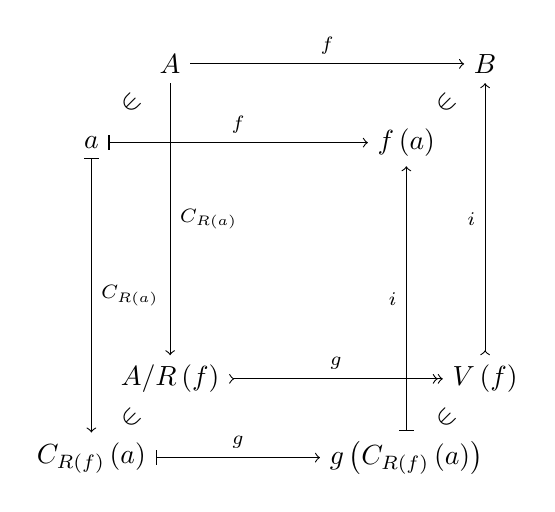
\begin{tikzpicture}[auto] 

  \node (a) at (1, 1) {$A/R\left( f\right) $};
  \node (b) at (5, 1) {$V\left( f\right) $};
  \node (c) at (0, 0) {$C_{R\left( f\right) } \left( a\right) $};
  \node (d) at (4, 0) {$g\left( C_{R\left( f\right) } \left( a\right) \right) $};
  \node (f) at (1, 5) {$A$};
  \node (g) at (5, 5) {$B$};
  \node (h) at (0, 4) {$a$};
  \node (i) at (4, 4) {$f\left( a\right) $};
  \node (e) at (0.5, 4.5) {\rotatebox{45}{$\in $} };
  \node (e) at (4.5, 4.5) {\rotatebox{45}{$\in $} };
  \node (e) at (0.5, 0.5) {\rotatebox{45}{$\in $} };
  \node (e) at (4.5, 0.5) {\rotatebox{45}{$\in $} };
    
  \draw [->] (f) to node {$\scriptstyle C_{R\left( a\right) } $} (a);
  \draw [>->>] (a) to node {$\scriptstyle g$} (b);
  \draw [>->] (b) to node {$\scriptstyle i$} (g);
  \draw [->] (f) to node {$\scriptstyle f$} (g);
  \draw [|->] (h) to node {$\scriptstyle C_{R\left( a\right) } $} (c);
  \draw [|->] (c) to node {$\scriptstyle g$} (d);
  \draw [|->] (d) to node {$\scriptstyle i$} (i);
  \draw [|->] (h) to node {$\scriptstyle f$} (i);
  
\end{tikzpicture} 
\end{center}
\end{itemize}
その写像$g$を特にその写像$f$に付随する全単射ともいう。このようにして、その写像$f$がその写像$i \circ g \circ C_{R(f)}$に書き換えられることをその写像$f$の写像たち$C_{R(f)}$、$g$、$i$への分解などという\footnote{これは代数学とかでちょくちょく使うらしいです。}。
\end{thm}
\begin{proof}
写像$f:A \rightarrow B$とこれに付随するその集合$A$の同値関係$R(f)$が与えられたとき、写像$g$が次式のように定義される。
\begin{align*}
g:A/R(f)\rightarrow V(f);C_{R(f)}(a) \mapsto f(a)
\end{align*}
このとき、定義より明らかに$V(g) \subseteq V(f)$が成り立つ。ここで、、$\forall f(a) \in V(f)$に対し、値域の定義より$f(a) \in V(f)$なる元$a$がその集合$A$に存在する。この元$a$に対し、明らかに同値類$C_{R(f)}(a)$がその集合$A/R(f)$に存在することになるので、$f(a) = g\left( C_{R(f)}(a) \right)$なる同値類$C_{R(f)}(a)$がその集合$A/R(f)$に存在することになる。したがって、次式が成り立ち
\begin{align*}
f(a) \in V(f) \land \exists C_{R(f)}(a) \in A/R(f)\left[ f(a) = g\left( C_{R(f)}(a) \right) \right]
\end{align*}
値域の定義より$f(a) \in V(g)$が成り立つので、$V(f) \subseteq V(g)$が得られる。以上より、$V(g) = V(f)$が成り立つので、その写像$g$は全射である。また、$\forall C_{R(f)}(a),C_{R(f)}(b) \in A/R(f)$に対し、$C_{R(f)}(a) \neq C_{R(f)}(b)$が成り立つなら、$aR(f)b$が成り立たないので、その写像$f$に付随する同値関係の定義より$f(a) \neq f(b)$が成り立つ。したがって、$g\left( C_{R(f)}(a) \right) \neq g\left( C_{R(f)}(b) \right)$が成り立つことになるので、その写像$g$は単射である。以上より、その写像$g$は全単射であることが示された。\par
また、その集合$A$からその集合$A/R(f)$への標準的全射$C_{R(f)}$とその集合$V(f)$からその集合$B$への標準的単射$i$が与えられたとすれば、$\forall a \in A$に対し、次式が成り立つ。
\begin{align*}
i \circ g \circ C_{R(f)}(a) = i\left( g\left( C_{R(f)}(a) \right) \right) = i\left( f(a) \right) = f(a)
\end{align*}
したがって、その写像$f$はその集合$A$からその集合$A/R(f)$への標準的全射$C_{R(f)}$とその写像$g$とその集合$V(f)$からその集合$B$への標準的単射$i$を用いた次式を満たす。
\begin{align*}
f = i \circ g \circ C_{R(f)}
\end{align*}
\end{proof}
\begin{thebibliography}{50}
\bibitem{1}
  松坂和夫, 集合・位相入門, 岩波書店, 1968. 新装版第2刷 p39-60 ISBM978-4-00-029871-1
\end{thebibliography}
\end{document}
